\documentclass[tikz,border=3pt]{standalone}
\usepackage[T1]{fontenc}
\usepackage{helvet}
\renewcommand{\familydefault}{\sfdefault}
\usetikzlibrary{arrows.meta,fit,calc}

\tikzset{
  stage/.style={draw, line width=0.9pt, inner sep=3.5mm},
  block/.style={draw, line width=0.65pt, align=center, minimum height=9mm, inner sep=1.5mm},
  subblock/.style={draw, line width=0.5pt, align=center, minimum height=8mm, inner sep=1.2mm},
  flow/.style={-{Latex[length=2.1mm,width=1.45mm]}, line width=0.75pt},
  legacy/.style={flow, dashed, dash pattern=on 3mm off 2mm},
  stage title/.style={font=\bfseries\small},
  path label/.style={font=\bfseries\scriptsize, fill=white, inner sep=1pt}
}

\begin{document}
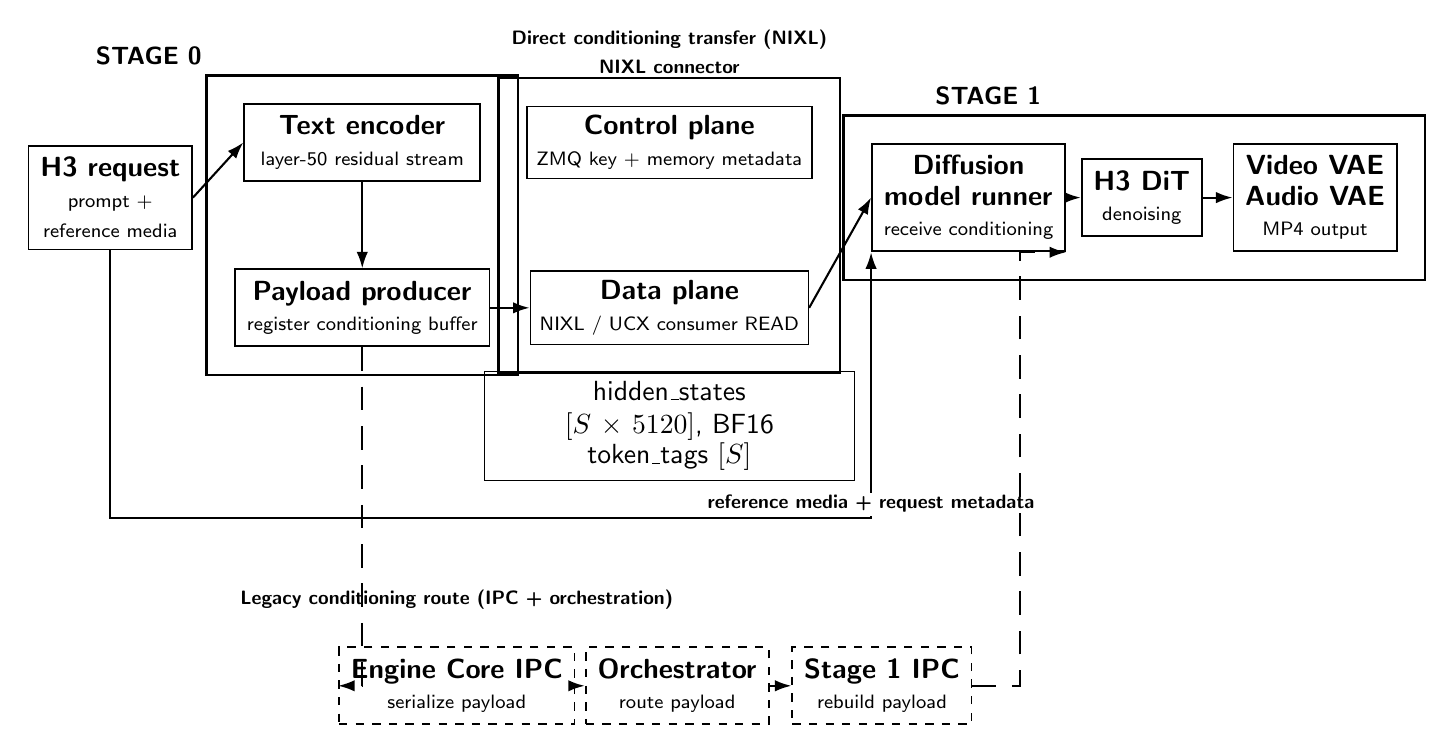
\begin{tikzpicture}[x=1mm,y=1mm]
  \node[block, minimum width=18mm] (request) at (-5,0)
    {\textbf{H3 request}\\[-1pt]\scriptsize prompt +\\[-1pt]\scriptsize reference media};

  \node[block, minimum width=30mm] (encoder) at (27,7)
    {\textbf{Text encoder}\\[-1pt]\scriptsize layer-50 residual stream};
  \node[block, minimum width=30mm] (producer) at (27,-14)
    {\textbf{Payload producer}\\[-1pt]\scriptsize register conditioning buffer};
  \node[stage, fit=(encoder)(producer), label={[stage title]above left:STAGE 0}] (stage0) {};

  \node[subblock, minimum width=28mm] (control) at (66,7)
    {\textbf{Control plane}\\[-1pt]\scriptsize ZMQ key + memory metadata};
  \node[subblock, minimum width=28mm] (data) at (66,-14)
    {\textbf{Data plane}\\[-1pt]\scriptsize NIXL / UCX consumer READ};
  \node[stage, fit=(control)(data), label={[path label]above:NIXL connector}] (connector) {};

  \node[block, minimum width=22mm] (runner) at (104,0)
    {\textbf{Diffusion}\\[-1pt]\textbf{model runner}\\[-1pt]\scriptsize receive conditioning};
  \node[block, minimum width=13mm] (dit) at (126,0)
    {\textbf{H3 DiT}\\[-1pt]\scriptsize denoising};
  \node[block, minimum width=18mm] (vae) at (148,0)
    {\textbf{Video VAE}\\[-1pt]\textbf{Audio VAE}\\[-1pt]\scriptsize MP4 output};
  \node[stage, fit=(runner)(dit)(vae), label={[stage title]above left:STAGE 1}] (stage1) {};

  \draw[flow] (request.east) -- (encoder.west);
  \draw[flow] (encoder) -- (producer);
  \draw[flow] (producer.east) -- (data.west);
  \draw[flow] (data.east) -- (runner.west);
  \draw[flow] (runner) -- (dit);
  \draw[flow] (dit) -- (vae);

  \node[path label] at (66,20) {Direct conditioning transfer (NIXL)};
  \node[subblock, minimum width=47mm, text width=43mm] (payload) at (66,-29)
    {hidden\_states $[S \times 5120]$, BF16\\[-1pt]token\_tags $[S]$};

  \draw[flow] (request.south) -- ++(0,-34) -|
    node[path label, pos=0.56, below=2pt] {reference media + request metadata}
    (runner.south west);

  \node[block, dashed, minimum width=23mm] (engineipc) at (39,-62)
    {\textbf{Engine Core IPC}\\[-1pt]\scriptsize serialize payload};
  \node[block, dashed, minimum width=20mm] (orchestrator) at (67,-62)
    {\textbf{Orchestrator}\\[-1pt]\scriptsize route payload};
  \node[block, dashed, minimum width=21mm] (stageipc) at (93,-62)
    {\textbf{Stage 1 IPC}\\[-1pt]\scriptsize rebuild payload};

  \node[path label] at (39,-51) {Legacy conditioning route (IPC + orchestration)};
  \draw[legacy] (producer.south) |- (engineipc.west);
  \draw[legacy] (engineipc) -- (orchestrator);
  \draw[legacy] (orchestrator) -- (stageipc);
  \draw[legacy] (stageipc.east) -- ++(6,0) |- (runner.south east);
\end{tikzpicture}
\end{document}
